\chapter{相关研究进展}
\section{引言}
自从计算机技术应用到医学影像分析以来,有许许多多医学影像分析难题因其具有的重大临床应用价值和实际意义而引起研究者的浓厚兴趣并为之投入大量时间和精力,生物标记物的精确定位便是其中之一。本章将会生物标记物精确定位任务的常用数据集进行介绍。接着将会介绍本文方法中涉及到的最为重要的基本知识点,包括卷积神经网络、对抗生成网络和自编码-解码器等。下一步,我们将对可用于完成生物标记物精确定位任务的已有解决方案进行详细(包括传统的多示例学习和当下流行的卷积神经网络方法)介绍,力求将相关方法阐述得清晰明了,突出比较各种方法在生物标记物的精确定位任务上的长处和不足。在本章最后,我们将给出实验结果的评判标准,并阐述选择这些比较标准的合理性。

\section{常用数据集}
一旦展开对选取问题的具体研究,第一步便是选取实验所使用的数据集。尤其对于当下十分火热、有着数据驱动特性的卷积神经网络来说,选择一个合适的数据集的重要性更加不言而喻。再加上医学影像数据获取、标注成本更高,导致可用于生物标记物的精确定位测试的公开数据集较少。由于医学数据很可能会涉及到病人的隐私,为了尽可能保护病人权益,防止病人信息泄露,图像数量较多的、图像质量较高的数据集往往存于知名公立医院且未公开。在已然公开的数据集中,本文将选取一些知名度较高的、在学术界被研究者广泛接受的、图像质量相对较高的数据集进行介绍。

\subsection{眼底病变数据集}
眼科学是临床医学的一个独特分支。眼科的影像学检查方法有眼底摄影、光学相干断层扫描、眼底荧光血管造影、扫描激光检眼镜等。一个明确的眼科疾病诊断需要结合几个不同的试验结果。在临床实践中,诊断和治疗策略的确定依赖于影像学资料的评价。目前眼底照片已广泛应用于青光眼和视网膜疾病等眼科疾病的诊断。然而,眼成像数据的解释需要大量的经验和时间。在这里,我们介绍部分具有良好注释和标签的数据集,扼要信息如表~\ref{tab:datasets_info}所示,下面分别进行简单介绍。
\begin{table}[h]
	\centering
	\caption{常用眼底病变数据集。}		
	\label{tab:datasets_info}
	\begin{tabular}{c|c|c|c}
		\toprule[2pt]
		数据集名称 & 图像数量 & 类别 & 标注 \\
		\midrule[2pt]
		Kaggle Diabetic Retinopathy (DR)	& 35,127	& 5	&图像级 \\
		\hline                         
		iChallenge Glaucomatous Optic Neuropathy (GON)    & 1,200    & 2 & 图像级 \\ \hline
		iChallenge Age-related Macular Degeneration (AMD) & 1,200    & 2 & 部分像素级 \\ \hline
		iChallenge Pathological Myopia (PM)               & 1,200    & 2 & 部分像素级 \\ \hline
		ODIR-5K & 7,000 & 8 & 图像级 \\ \hline
		
		Indian Diabetic Retinopathy Image Dataset (IDRiD) & 516 & 5 & 部分像素级 \\
		\bottomrule[2pt]
	\end{tabular}
\end{table}

注意,图像级标注指的是将图像标注为对应类别,如正常/异常。像素级标注在图像级标注基础上还标出病变的准确位置。另外,图像数量指的是数据集中官方有提供标注的图像数据。以上说明同样适用于表~\ref{tab:skin_datasets_info}。

糖尿病视网膜病变是发达国家劳动年龄人口失明的主要原因。DR数据集\footnote{https://www.kaggle.com/c/diabetic-retinopathy-detection/data}是目前关于糖尿病视网膜病变的最大数据集,提供了在各种成像条件下拍摄的高分辨率视网膜图像。目前在Kaggle上开源数据中,训练集有35,127张样本,每张图像尺寸均大于$1000\times 1000$但大小不等,目前只有图像集标注。专业医师根据患者患病程度将每张图像标注为0至4共5类。0、1、2、3和4分别代表未患糖尿病视网膜病变、轻微糖尿病视网膜病变、中度糖尿病视网膜病变、严重糖尿病视网膜病变和增生性糖尿病视网膜病变。标注数字越大代表患病越严重。

GON数据集\footnote{http://ai.baidu.com/broad/subordinate?dataset=gno}是关于青光眼眼底照片的数据集,共包含1,200张彩色眼底照片。并平均分为训练集、验证集和测试集。其中,训练集图像由德国蔡司眼底照相机拍摄,尺寸大小为$2124\times 2056$,验证集和测试集图像由佳能眼底照相机拍摄,尺寸大小为$1634\times 1634 $。所有图像均是图像集标注,标记为青光眼/非青光眼,均以后极为中心,伴有黄斑和视盘。

AMD数据集\footnote{http://ai.baidu.com/broad/subordinate?dataset=amd}是关于年龄相关性黄斑变性眼底照片数据库,共有1,200张彩色眼底照片可供选择。这些照片来自非AMD受试者(约77\%)和AMD患者(约23\%)。提供AMD/非AMD的标签,椎间盘边界和中央凹的位置,以及各种病变的边界,以训练模型进行自动AMD评估。数据集中每个样本都有图像级标注,只有部分样本有像素级标注,标注了与年龄相关性黄斑变性相关的四种典型异常。

近视已成为全球公共卫生的负担。为了促进近视的研究,PM数据集\footnote{http://ai.baidu.com/broad/subordinate?dataset=pm}是病理性近视眼底照片数据库,提供了1200个来自非病理性近视受试者和病理性近视患者(约50\%)的标注视网膜眼底图像的大数据集。每个图像样本同样均有图像级标注,部分图像有包括斑片状视网膜萎缩(包括乳头周围萎缩)和视网膜脱离在内的两种典型异常的像素级标注。

ODIR-5K数据集\footnote{https://odir2019.grand-challenge.org/dataset/}是一个结构化的眼科数据库,其中包括5,000名患有年龄的患者,双眼的彩色眼底照片和医生的诊断关键词。注意只有3,500名患者(7,000张样本)数据作为训练集,并且有图像级标签。该数据集是上工医疗技术有限公司从中国不同医院/医疗中心收集的“真实”患者信息。专业医师将患者分为8个标签,包括正常,糖尿病,青光眼,白内障,年龄相关性黄斑变性,高血压,近视和其他疾病/异常。由于存在部分病人同时患有多种疾病,因而部分图像有多个标签。

IDRiD\footnote{https://idrid.grand-challenge.org/Data/}眼底图像是由印度一家眼科诊所的视网膜专家收集的。数据集共包括516张样本,均提供了典型糖尿病视网膜病变病变和正常视网膜结构的专家标记。数据集所有图像都集中在黄斑附近。图像分辨率为$4288\times 2848$像素,存储为jpg文件格式。此外,它还根据国际临床相关性标准,为数据库中的每张图像提供关于糖尿病视网膜病变的疾病严重程度和糖尿病黄斑水肿的信息。与DR数据集一样,它一共将图像分为5类。与DR数据集不同的是,IDRiD数据集有81张患病彩色眼袋图像有精确像素级标注,如微动脉瘤、软渗出物、硬渗出物和出血。

眼底病变往往有病变区域较小,病变区域数量较多,病变区域分布较分散的特点。因此,眼底有些病变区域容易混淆,比较难发现。另外,眼底图像较为精细,各种细节纹理丰富,故发现眼底病变的生物标记物通常极具挑战性。

\subsection{黑色素瘤皮肤病变图像}
黑色素瘤是多种皮肤癌中最致命的一种。黑色素瘤是发生在皮肤表面的色素性病变,可以通过专业医师的视觉检查早期发现。黑色素瘤也适用于自动检测与图像分析。皮肤镜检查是一种皮肤成像方法,与无辅助的视觉检查相比,已证明可改善皮肤癌的诊断。为了更广泛地提供专业知识,国际皮肤成像协作组织开发了专门档案,这是一个国际皮肤镜图像库,可用于皮肤科专业医师的临床培训,也能用于举办比赛,寻求计算机算法解决临床问题。在这里,我们介绍三个图像质量较高,可用于生物标记物定位的黑色素瘤病变数据集。数据集名称、图像数量等基本信息如表~\ref{tab:skin_datasets_info}所示。


\begin{table}[h]
	\centering
	\caption{常用眼底病变数据集。}		
	\label{tab:skin_datasets_info}
	\begin{tabular}{c|c|c|c}
		\toprule[2pt]
		数据集名称 & 图像数量 & 类别 & 标注 \\
		\midrule[2pt]
		
		International Skin Imaging Collaboration (ISIC) 2017 &  $\sim 2,300$ & 3 & 部分像素级 \\ \hline
		International Skin Imaging Collaboration (ISIC) 2018 & $\geq 12,500$ & 7  & 部分像素级 \\ \hline
		International Skin Imaging Collaboration (ISIC) 2019 & 25,331 & 8  & 图像级  \\ 
		\bottomrule[2pt]
	\end{tabular}
\end{table}

ISIC2017数据集~\cite{codella2018skin}中大约有2,300张皮肤镜图像,其中大约2,150张图像是训练集,剩下约150张图像是验证集。图像尺寸大小在$400\sim 600$之间。数据集包括黑色素瘤、脂溢性角化病和良性的痣(可看做正常)在内的3种类别。

ISIC2018数据集~\cite{codella2019skin, tschandl2018ham10000}中有超过12,500张皮肤镜图像。图像尺寸大小在$400\sim 600$之间。包括光化性角化病(日光性角化病)和上皮内癌(鲍文氏病)、基底细胞癌、良性的角化病、皮肤纤维瘤、黑素细胞痣、黑素瘤、血管皮肤损伤共7类。

ISIC2019数据集\footnote{https://challenge2019.isic-archive.com/}中有25,331张皮肤镜图像,包括黑色素瘤黑素细胞痣、基底细胞癌、光化性角化病、良性角化病(太阳扁豆/脂溢性角化病/扁平苔藓样角化病)、皮肤纤维瘤、血管病变、鳞状细胞癌和没有以上病变类型在内的8个类别。图像尺寸大小在$400\sim 600$之间。

与眼底病变类型不同的是,黑色素瘤的各种病变类型往往在皮肤镜上所占区域比较大,通常所占比例在$1/3$以上。各种病变类型之间的区别主要表现在病变区域细微纹理区间上。

\section{基本知识要点}
本小节主要是介绍生物标记物定位任务的概念和目前常用的模型方法。首先,我们会介绍生物标记物定位任务的概念,让读者对本文研究主题有清晰的认识。接着会介绍卷积神经网络、编码器-解码器等重要基本要点。下一步介绍目前已有的常用解决模型方法。最后介绍对各种模型方法性能比较的评价标准。
\subsection{生物标记物定位任务}
\begin{figure}[h]
	\centering
	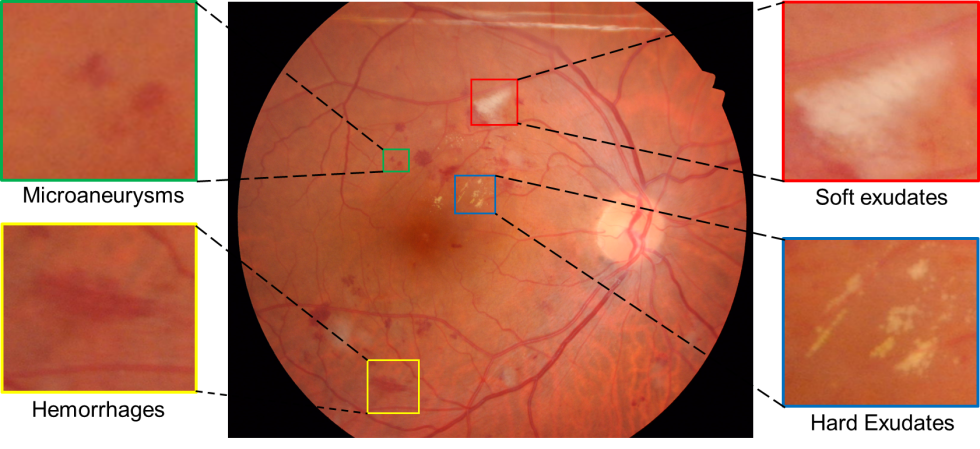
\includegraphics[width=1.0\textwidth]{figure/biomarker_localization_example}
	\caption{生物标记物定位任务示例。红色矩形框、绿色矩形框、蓝色矩形框和黄色矩形框标记了四种糖尿病视网膜病变的异常表现,分别代表软性渗出液(Soft Exudates)、微动脉瘤
		(Microaneurysms)、硬性渗出液(Hard Exudates)和出血(Hemorrhages)。} 
	\label{fig:biomarker_localization_example}
\end{figure}
生物标志物是开发新疗法和辅助诊断的关键,受到研究人员的不断关注,其目标是为合适的病人开发合适的药物。随着计算机视觉技术不断应用到医学领域,生物标记物定位任务自然也变成了研究热点。在医学影像处理领域,一旦一张医学影像被诊断为某种特定疾病,生物标记物定位任务的目标便是寻找其患病区域,或者说在图像上找到诊断依据,该依据或者患病区域即可看作是生物标记物。如图\ref{fig:biomarker_localization_example},该图像被诊断为患有糖尿病视网膜病变,生物标记物定位任务便是找到其异常表现,并给出其准确位置。可以发现,糖尿病视网膜病变有多种异常表现,生物标记物定位任务要求不能漏检。另外,可以发现从颜色特征上看,出血(图中黄色矩形框)异常和眼底血管非常相似,因而将微小血管看作异常表现的假阳现象也可能发现。以上均给生物标记物定位任务增加了不少难度。如果将卷积神经网络手段,根据以上介绍,生物标记物定位任务的目标是找出疾病诊断背后的诊断依据,这与卷积神经网络的可视化/可解释性的目标恰好一致,因此卷积神经网络的可视化/可解释性是生物标记物定位任务的主要解决方案之一。相关内容将会在\ref{subsec:visulization_methods}小节详细叙述。
\subsection{卷积神经网络}
卷积神经网络最初是为了避免传统神经网络(多层感知机~\cite{gardner1998artificial})在处理图像时的缺点而提出的。多层感知机在处理图像数据时,多层感知机对每张输入图像中的每个像素点都使用一个感知器。对于较大的图像,权重的数量很快就变得难以管理。例如,对于一个有3个彩色通道的224$\times$224像素图像,大约需要训练150,000个权值。此时,多层感知机的训练将变得十分困难。另外,多层感知机不具备平移不变性。例如,如果一张猫出现在一张图像的左上角和另一张图像的右下角,多层感知机将假设猫总是出现在图片的这个位置。再加上,多层感知机在处理图像时需要将二维图像数据将会以一维向量形式存在,因此无法利用二维空间的相对位置信息。
\begin{figure}[h]
	\centering
	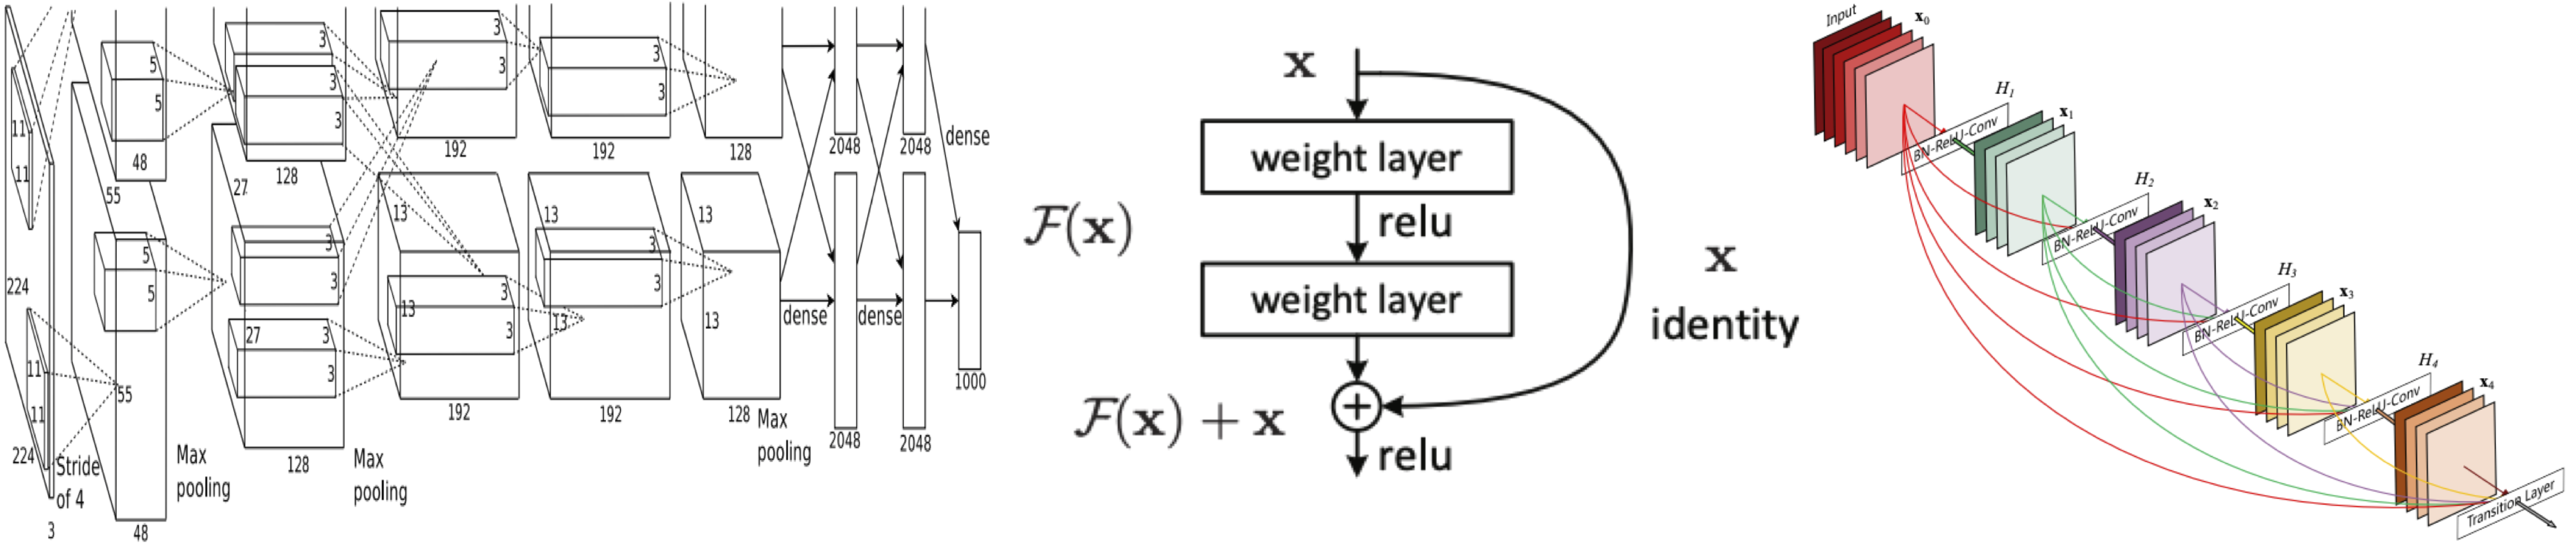
\includegraphics[width=1.0\textwidth]{figure/popular_networks}
	\caption{三种经典的卷积神经网络模型结构。从左到右,依次为AlexNet~\cite{krizhevsky2012imagenet}、ResNet~\cite{he2016deep, he2016identity}、DenseNet~\cite{huang2017densely}(图片均来自于原始论文)。注意,中间是ResNet的一个残差单元,ResNet实际上是由多个残差单元堆叠组成。} 
	\label{fig:popular_networks}
\end{figure}

卷积神经网络便可以很好避免多层感知机存在的问题,卷积操作可以很好的捕捉图像的空间信息。另外,卷机操作还具有平移不变性。权值共享机制可以大大降低参数量。随着计算机算力的快速提升,运用反向传播算法~\cite{hecht1992theory},卷积神经网络的大规模训练变得切实可行。自Hinton等人利用两块GPU成功训练AlexNet~\cite{krizhevsky2012imagenet}后,很多优秀网络结构被提出,比如VGG~\cite{simonyan2014very},ResNet~\cite{he2016deep, he2016identity},DenseNet~\cite{huang2017densely},Inception系列网络~\cite{szegedy2015going, szegedy2016rethinking, szegedy2017inception}。卷积神经网络除了在分类问题上取得出色性能外,还在自然语言处理~\cite{dos2014deep, mou2016convolutional, li2019knowledge}、无人驾驶~\cite{lee2017deep, csillik2018identification, tang2017vehicle}、语音识别~\cite{abdel2013exploring, swietojanski2014convolutional, robertson2019exploring}等领域表现不凡,越来越受到研究者们的青睐。

三种经典的卷积神经网络的模型结构如图~\ref{fig:popular_networks}所示。可以看出,卷积神经网络都是由一系列卷积操作组成的,在卷积操作之后再接上激活函数以增强非线性表达能力。为了减少参数量,卷积神经网络还引入了池化操作,使得输入图像尺寸随着深度不断增加而减小。池化操作也起到过滤无用信息的的作用。最后,再接上全连接层对卷积神经网络提取到的特征进行分类(视不同任务而改变)。因此,卷积神经网络实际上充当特征提取器的角色。那么我们可以这样理解卷积神经的原理:单纯卷积操作提取的是图像的局部信息,随着一系列卷积操作的堆叠,卷积神经网络的感受野越来越大,比如两个3$\times$3的卷积核堆叠相当于一个5$\times$5卷积核的感受野,卷积神经网络便能提取到图像的全局信息。同时,随着深度增加,输入的尺寸大小变得越来越小,通常以2倍关系减小,卷积神经网络便会丢掉无用信息。因而卷积神经网络是一种层次化结构。再在损失函数,如交叉熵,的监督指导下,根据反向梯度传播算法更新网络参数,卷积神经网络便能被训练成一个优秀的特征提取器。

以上便是卷积神经网络的一般结构和工作原理,下面详细介绍ResNet。随着VGG-19~\cite{simonyan2014very}的出现,一个卷积神经网络的深度越深,学出来的效果是否越好的问题摆在了研究者们的面前。由于卷积神经网络的深度越深,原本就存在的过拟合和梯度消失问题变得越严重。何凯明等人便设计了一种在深度远大于VGG-19,效果也由于VGG-19的网络模型。设$\mathcal{H}(x)$是卷积神经网络拟合的函数,$x$表示网络输入。如果假设多个非线性层可以渐近逼近复杂函数并且假设输入和输出尺寸相同,那么就可以假设它们可以渐近逼近残差函数$\mathcal{F}(x)$,即$\mathcal{F}(x)=\mathcal{H}(x)− x$。因此,ResNet没有让网络直接拟合$\mathcal{H}(x)$,而是明确地让这些层近似为残差函数$\mathcal{F}(x)=\mathcal{H}(x)-x$。 因此,原始函数变为$\mathcal{F}(x)+x$。尽管两种形式都应能够渐近地逼近所需的功能(如假设),但是近似拟合残差函数要容易得多。另外,为了表示加号,残差单元中通常加入跳接操作。

设$x_l$表示第$l$个残差单元的输入,$\mathcal{W}_{l}=\{\mathcal{W}_{l,k}|_{1\leq k \leq K}\}$表示第$l$个残差单元的权重,$K$表示残差单元个数。则相邻的残差单元输入$x_{l+1}$可以表示为:
\begin{gather}
	y_{l}=x_l + \mathcal{F}(x_l, \mathcal{W}_l), \\
	x_{l+1}=f(y_{l}).
\end{gather}
其中$f$表示激活函数,$\mathcal{F}(x_l, \mathcal{W}_l)$表示残差单元中的卷积操作。如果$f$表示恒等变换,则$x_{l+1}=y_{l}$,有:
\begin{equation}
	x_{l+1}=x_l + \mathcal{F}(x_l, \mathcal{W}_l).
\end{equation}
对于任意第$L(L\ge l)$个残差单元,其输入$x_{L}$,可写为:
\begin{equation}\label{residual_block_compute}
x_{L}=x_l + \sum_{i=l}^{L-1}\mathcal{F}(x_i, \mathcal{W}_i).
\end{equation}
设损失函数为$\varepsilon$,根据等式\ref{residual_block_compute}和反向梯度传播算法的链式求导法有:
\begin{equation}\label{residual_block_gradient}
\frac{\partial \varepsilon}{\partial x_l}=\frac{\partial \varepsilon}{\partial x_L}\frac{\partial x_L}{\partial x_l}=\frac{\partial \varepsilon}{\partial x_L}(1+\frac{\partial}{\partial x_l}\sum_{i=l}^{L-1}\mathcal{F}(x_i,\mathcal{W}_i)).
\end{equation}
等式\ref{residual_block_gradient}表明,梯度$\frac{\partial \varepsilon}{\partial x_l}$由$\frac{\partial \varepsilon}{\partial x_L}$和$\frac{\partial \varepsilon}{\partial x_L}\frac{\partial}{\partial x_l}\sum_{i=l}^{L-1}\mathcal{F}(x_i,\mathcal{W}_i)$两项组成。第一项在可直接传播信息而与任意残差单元无关。而第二项保证信息直接回传到上一个残差单元。由于第一项的存在,等式\ref{residual_block_gradient}还能保证每一层梯度不容易消失,即使在残差单元权重很小的情况下。而ResNet更是实现了在深度达到上千层的情况下,仍不会发生梯度消失现象。DenseNet更是将ResNet中提出的跳接扩展到了网络单元之间,正是由于ResNet的优异性能,本文卷积神经网络分类器使用ResNet-18。
\subsection{编码器-解码器}
\begin{figure}[h]
	\centering
	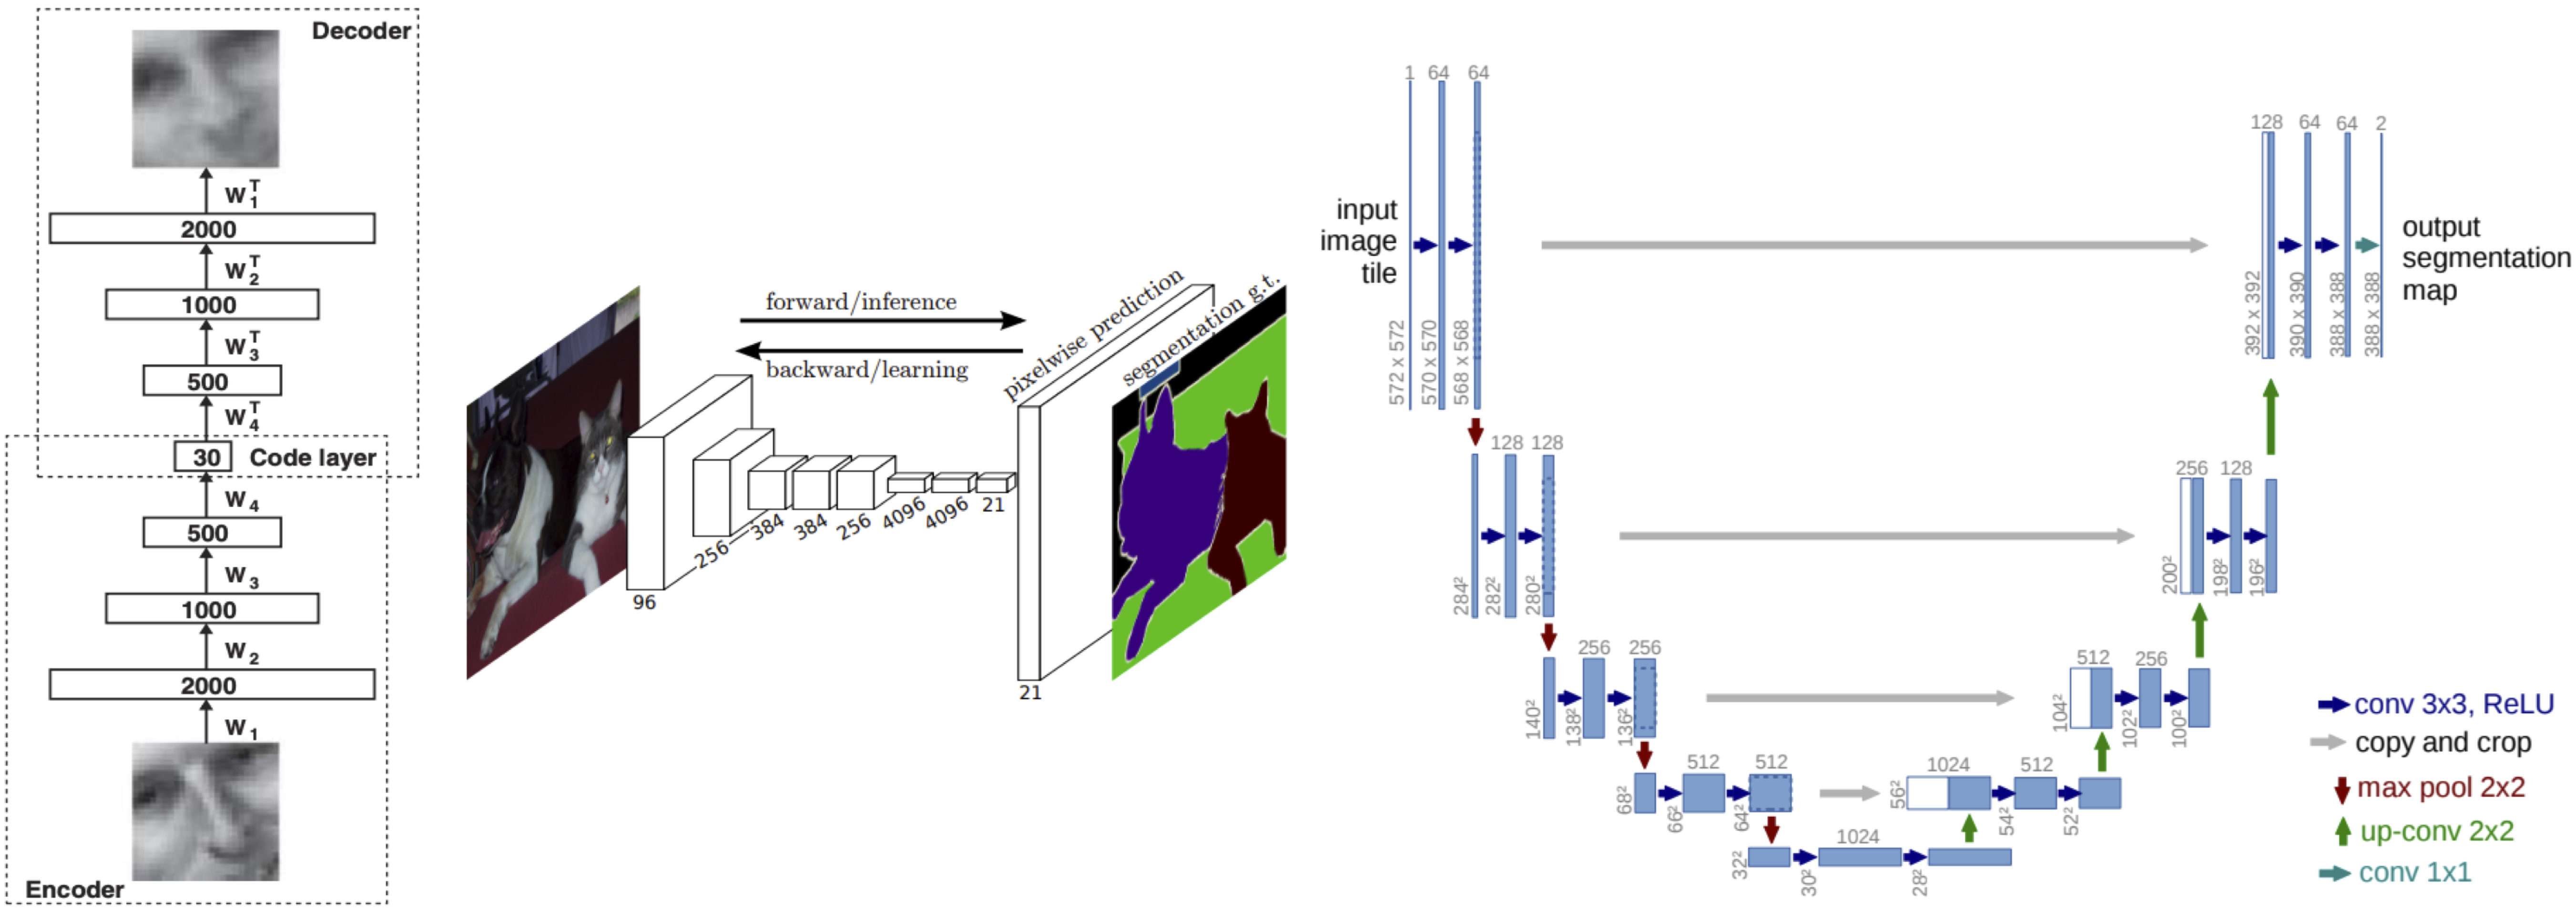
\includegraphics[width=1.0\textwidth]{figure/popular_encoder_decoder}
	\caption{三种经典的编码器-解码器模型结构。从左到右依次为编码器-解码器~\cite{hinton2006reducing}、全卷积神经网络~\cite{long2015fully}和U-Net~\cite{ronneberger2015u}(图片均来自于原文)。} 
	\label{fig:popular_encoder_decoder}
\end{figure}
编码-解码器自Hinton等人~\cite{hinton2006reducing}提出以来被广泛应用。编码-解码器不是某一种网络,而是代表了一类网络。随后便有降噪编码器-解码器~\cite{vincent2008extracting}、稀疏编码器-解码器~\cite{coates2011analysis}、变分贝叶斯编码器-解码器~\cite{kingma2013auto}等变体。将卷积操作应用到编码器-解码器中,启发了FCN~\cite{long2015fully}、U-Net~\cite{ronneberger2015u}、FPN~\cite{lin2017feature}等经典网络结构。FCN和U-Net均是分割分割领域(包括自然图像和医学图像)最为基础的网络结构。为了读者对编码器-解码器模型结构由较为直观的认识,三种经典网络结构如图\ref{fig:popular_encoder_decoder}所示。

在深度学学习领域,编码器-解码器是一种无监督的神经网络。从图\ref{fig:popular_encoder_decoder}可看出,编码器-解码器共同特点是由编码器和解码器组成,下面展开简要介绍:

1)编码器:编码器在网络结构图中是将卷积操作输入不断变小的过程,U-Net中是运用池化层实现下采样,不断将卷积操作输入以2倍关系缩小,从而达到提取图像特征的目的。由于通过编码器,可将输入维度不断降低,因此编码器-解码器最直观的应用便是图像压缩和图像去燥。在实际使用过程中,为了让编码器提取到输入较好的特征表达,通常会利用深度学习网络知识可迁移的优点,用Image-Net~\cite{deng2009imagenet}上的预训练模型参数来初始化编码器~\cite{iglovikov2018ternausnet}。

2)解码器:解码器和编码器相反,是将特征不断扩大,最终恢复到原图像大小的过程。通常会使用上采样或者反卷积~\cite{zeiler2010deconvolutional}操作以2倍关系逐步扩大,从而达到融合不同层次、不同尺寸的特征的目的。

由于本文使用到了U-Net~\cite{ronneberger2015u},故同时简单介绍U-Net。除了以上特点之外,U-Net中还存在从编码器直接到解码器的跨层连接,这些跨层连接使网络可以将上下文信息传播到更高分辨率的层,从而使得特征融合更加充分。在网络可视化图上(见图\ref{fig:popular_encoder_decoder}右子图),由于编码器和解码器相互对称,形成一个U型结构。U-Net中只含有卷积层,不含任何全连接层,最后视不同任务而接上不同激活函数。U-Net作为一种巧妙的网络模型,被广泛应用于医学影像处理领域~\cite{cciccek20163d, han2018framing, dong2017automatic, sevastopolsky2017optic, zhang2018ct},更多启发了诸多优秀网络模型~\cite{zhou2018unet++, oktay2018attention, ibtehaz2020multiresunet, alom2019recurrent, milletari2016v}。
\subsection{对抗生成网络}
对抗生成网络(Generative Adversarial Networks,缩写为GAN)最初于2014年由Goodfellow等人~\cite{goodfellow2014generative}提出,就越来越受到学术界和工业界的重视。而随着GAN在理论与模型上的高速发展,它在计算机视觉~\cite{zhu2017unpaired, isola2017image}、自然语言处理~\cite{qin2018dsgan, guimaraes2017objective}、人机交互~\cite{qiao2018emotional, sahu2018enhancing}等领域有着越来越深入的应用,在医学影像领域更是大放异彩~\cite{yang2017dagan, yang2018low, shin2018medical, onishi2020multiplanar, bhadra2020medical}。GAN是生成式模型,受博弈论中的零和博弈启发,将生成问题视作判别网络和生成网络这两个网络的对抗和博弈。生成网络努力生成新数据,判别器努力区分生成网络生成的数据(一般记为“假”)和真实数据(一般记为“真”)。生成网络尽量产生更真实的数据,而判别器尽量更完美地把真实数据与生成数据区分开来。由此,生成网络和判别器形成对抗关系,彼此进步。在不断的迭代训练过程中,生成网络生成的数据也就越来越逼近真实数据,即生成网络学到的分布越来越接近真实数据代表的分布。在理想情况下,判别器无法区分生成的数据和真实的数据。

设真实数据为$x\sim p_{data}(x)$,噪音为$z\sim p_z(z)$,生成网络和判别网络分别用$G$和$D$表示。$\theta_{g}$和$\theta_{d}$分表表示$G$和$D$的训练参数。则$G(z;\theta_{g})$表示生成网络生成的函数映射。$D(x;\theta_{d})$将会输出一个数值。可将$D$看做一个二类分类器。不妨将交叉熵当做损失函数。因此,可用$D(x)(0\leq D(x)\leq 1)$表示数据$x$来自于真实数据的概率。运用极大极小优化理论,GAN的损失函数可写成:
\begin{equation}\label{equ:gan_loss_func}
\min _{G} \max _{D} V(D, G)=\mathbb{E}_{\boldsymbol{x} \sim p_{\text {data }}(\boldsymbol{x})}[\log D(\boldsymbol{x})]+\mathbb{E}_{\boldsymbol{z} \sim p_{\boldsymbol{z}}(\boldsymbol{z})}[\log (1-D(G(\boldsymbol{z})))].
\end{equation}
我们对$D$进行训练,使其对$G$中的训练示例和样本分配正确标签的概率最大化。我们同时对$G$进行训练,使其对$log(1 - D(G(z))$最小化。换句话说,$D$和$G$玩了一个具有损失函数$V (G, D)$的二人极大极小博弈。在实际训练时,$D$和$G$先后交替训练。

\noindent 固定$\theta_{g}$,优化$\theta_{d}$等价于用随机梯度上升算法最大化损失函数:
\begin{equation}\label{equ:g_updated_loss_func}
\log D\left(x\right)+\log \left(1-D\left(G\left(z\right)\right)\right).
\end{equation}

\noindent 固定$\theta_{d}$,优化$\theta_{g}$等价于用随机梯度下降算法最小化损失函数:
\begin{equation}
\log \left(1-D\left(G\left(z\right)\right)\right).
\end{equation}
\noindent 在Goodfellol提出以上朴素GAN在生成网络和判别网络均是多层感知机。在实际训练过程中参数过大,训练难度较大的问题,因而训练不稳定,经常训练失败。各种改进模型相继提出,DCGAN~\cite{radford2015unsupervised}利用了卷积神经网络强大的拟合能力和容量。针对训练过程中存在的梯度消失问题,WGAN~\cite{gulrajani2017improved}使用Wasserstein-1距离代替GAN~\cite{goodfellow2014generative}中的Jensen-Shannon散度~\cite{arjovsky2017towards}。WGAN-GP~\cite{gulrajani2017improved}更是在WGAN基础上又在GAN损失函数(见等式\ref{equ:gan_loss_func})中加入了梯度惩罚项(Gradient Penalty),这也是WGAN-GP名字的由来。由于WGAN-GP可以有效避免GAN训练过程中的梯度消失,本文网络模型中GAN采用的就是WGAN-GP,下面进行简单简单介绍。

与朴素GAN~\cite{goodfellow2014generative}不同的是,在WGAN-GP中,判别器不再被看作是二分类器,而是近似去拟合Wasserstein-1距离,属于回归任务,因此也会去掉朴素GAN中判别器最后一层的Sigmoid激活函数。设$p_g$表示给定噪音分布$z\sim p_z$时生成网络所代表的的分布。再加上梯度惩罚项,WGAN-GP的损失函数可写作:
\begin{equation}\label{wgan_gp_loss_func}
\min _{G} \max _{D} V(D, G)=E_{x \sim P_{d a t a}}[D(x)]-E_{x \sim p_{g}}[D(x)]+\lambda E_{\hat{x} \sim p_{\hat{x}}}\left[\left(\left\|\nabla_{\hat{x}} D(\hat{x})\right\|_{2}-1\right)^{2}\right].
\end{equation}
其中,$\lambda$为梯度惩罚项的权重,分布$p_{\hat{x}}$不是对整个样本空间采样,而只对分布$p_{data}$和分布$p_{g}$之间的空间采样。在训练时同样$D$和$G$先后交替训练。因此,固定$G$,更新$\theta_{d}$时,等效于最小化损失函数:
\begin{gather}
\tilde{{x}} = G_{}({z}), \\
D(\tilde{{x}})-D({x})+\lambda\left(\left\|\nabla_{\hat{x}} D(\hat{x})\right\|_{2}-1\right)^{2}.
\end{gather}
\noindent 固定$D$,更新$G$时,等效于最小化损失函数:
\begin{equation}
-D\left(G_{\theta}(z)\right).
\end{equation}
通过实验证明,WGAN-GP在训练过程中梯度较为稳定,不易发生梯度消失现象。另外,Wasserstein-1距离还能指示WGAN-GP训练效果的作用,Wasserstein-1距离越大,表示WGAN-GP训练得越好,使得训练过程易于理解。
\section{生物标记物定位方法}
随着计算机计算在医学影像领域的广泛应用,目前已有可用于生物标记物定位的模型提出,主要包括多示例学习~\cite{maron1998framework}和卷积神经网络的可视化方法~\cite{zhou2016learning, selvaraju2017grad}。本小节将对其中的经典方法进行详细介绍,并比较方法之间的优劣,以便于读者对这些方法有清晰的认识与理解。
\subsection{多示例学习}
多示例学习~\cite{maron1998framework}
\subsection{卷积神经网络的可视化}\label{subsec:visulization_methods}
%\section{评价标准}
%\section{本章小结}